\documentclass[a4paper,12pt]{report}
\usepackage[T1]{fontenc}
\usepackage[latin1]{inputenc}
\usepackage[italian]{babel}
\usepackage{geometry}
\usepackage{graphicx}
\geometry{a4paper,top=3cm,bottom=3cm,left=2cm,right=2cm,heightrounded,bindingoffset=5mm}

\begin{document}

\author{Paolo Compagnoni}
\title{Specifiche del software per la gestione della consegna delle buste della raccolta differenziata
comune di Sant'Egidio alla Vibrata (TE)}

\maketitle

\tableofcontents

\newpage

Si intende progettare un software per informatizzare il servizio della raccolta differenziata del comune di Sant'Egidio alla Vibrata (TE).

\chapter{Descrizione del dominio applicativo}

Il comune di Sant'Egidio alla Vibrata distribuisce presso la biblioteca comunale buste, bidoni e calendari necessari per il corretto funzionamento della raccolta differenziata dei rifiuti. \newline
Per avere accesso al servizio, l'utente deve essere iscritto nell'elenco delle utenze TARI sia nel caso in cui esso sia un privato o un titolare/rappresentante di un'impresa. Nel caso in cui il cittadino non dovesse risultare negli elenchi, il servizio viene erogato comunque ma viene effettuato un controllo con l'ufficiale comunale che provveder� a verificare lo stato dell'utenza TARI. Se l'utente non risulta in regola, il servizio non verr� pi� erogato all'utente fino a quando esso risulta corretamente iscritto nell'elenco TARI.  \newline
Inoltre, la norma richiede che tra una consegna e l'altra delle buste deve passare almeno un mese e mezzo salvo richieste particolari dell'utente in periodi di maggiore necessit�. \newline
Esistono varie tipologie di bidoni per la raccolta differenziata che variano in base alla capienza. Per la consegna dei mastelli non occorrono particolari accertamenti mentre per gli altri bidoni, occorre verificarne l'effettiva necessit� tramite sopralluoghi.
Una volta che � stata verificata la necessit� del bidone richiesto, l'impiegato comunale accorda con l'utente le modalit� di consegna del bidone.
Infine, l'impiegato comunale a fine giornata deve verificare che il numero di rotoli, calendari e secchi sia uguale a quello presente nel programma. Nel caso in cui ci� non accada, bisogna annotarlo all'interno del programma.

\section{Utenti}

Le diverse tipologie di utenti che possono richiedere il servizio sono:
\begin{itemize}
\item Privato
\item Titolare/rappresentante di un'impresa
\end{itemize}

I \textbf{privati} hanno diritto ad un rotolo di buste per tipologia fatta eccezione per i rotoli per l'indifferenziato (colore rosso). Infatti nel caso in cui l'utente privato abbia particolari esigenze (ad esempio un anziano con particolari necessit� o bambini) possono essere consegnati due rotoli di buste per l'indifferenziato. \newline
Inoltre, ai privati vengono distribuiti solo i mastelli in caso di rottura accindentale o furto degli stessi. \newline \newline \newline \newline

I \textbf{titolari/rappresentanti di un'impresa} hanno diritto a massimo tre rotoli per tipologia di busta e possono richiedere bidoni di maggiori dimensioni. \newline \newline

Per ciascuna tipologia di utente vengono memorizzate le seguenti informazioni:

\begin{itemize}
\item Ragione sociale
\begin{itemize}
\item Cognome e nome, nel caso di persona fisica
\item Denominazione, nel caso di persona giuridica
\end{itemize}
\item Indirizzo
\end{itemize}

\section{Tipologie di rotoli}
Esistono quattro tipologie di rotoli, una per ogni tipologia di rifiuto:

\begin{itemize}
\item Indifferenziato (colore rosso)
\item Plastica (colore blu)
\item Carta (colore bianco)
\item Indumenti (colore verde)
\end{itemize}

\section{Tipologie di secchi}
Esistono quattro tipologie di secchi suddivisi per tipologia di utente:

\begin{itemize}
\item Per privati e condomini con meno di sei nuclei familiari:
\begin{itemize}
\item Mastelli
\end{itemize}
\item Per aziende:
\begin{itemize}
\item Bidoni da 300 litri
\item Bidoni da 700 litri
\item Bidoni da 1000 litri
\end{itemize}
\end{itemize}

\section{Organizzazione logistica}
Il magazzino dove viene conservato tutto ci� che viene fornito al cittadino (rotoli, calendari e secchi) viene immagazzinato al Centro Fiera che � situato a pochi chilometri dalla biblioteca comunale. In biblioteca � presente una piccola parte del materiale e viene conservato in una stanza apposita.

\chapter{Funzionalit� del programma}
Innanzitutto il programma permetter� la completa gestione delle utenze TARI, cio� si potr�:
\begin{itemize}
\item Consultare l'elenco TARI
\item Aggiungere un nuovo utente nell'elenco TARI
\item Modificare un utente dell'elenco TARI
\item Eliminare un utente dall'elenco TARI
\item Verificare che l'utente sia iscritto regolarmente nell'elenco TARI
\item Verificare che l'utente non abbia richiesto i rotoli prima di un mese e mezzo
\end{itemize}
In secondo luogo permetter� la gestione del magazzino, cio� si potr�:
\begin{itemize}
\item Consultare le quantit� rimaste nei due magazzini
\item Aggiornare le quantit� rimaste nei due magazzini
\item Notificare quando le scorte nei magazzini sono in esaurimento
\end{itemize}
Infine, il programma avr� alcune funzionalit� aggiuntive, cio� si potr�:
\begin{itemize}
\item Creare un elenco di utenti che non usufruiscono del servizio
\item Creare statistiche mensili e annuali in base al numero di richieste di rotoli, calendari e secchi
\end{itemize}

\chapter{Esempio di interfaccia grafica}

\begin{figure}
	\centering
		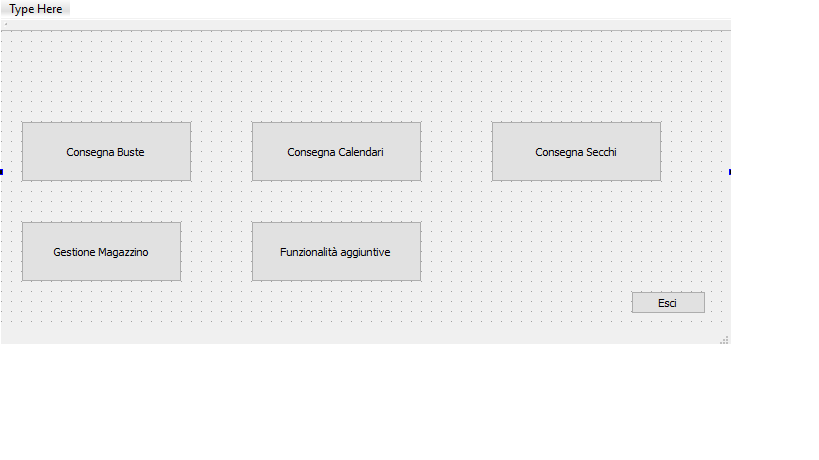
\includegraphics[scale=0.5]{Esempio_di_interfaccia.png}
	\label{fig:Esempio di interfaccia}
\end{figure}


\end{document}